\documentclass[11pt,a4paper]{article}

\usepackage[utf8]{inputenc}
\usepackage[cyr]{aeguill}
\usepackage[francais]{babel}

% Les packages
%\usepackage[french]{babel}
\usepackage{fancybox}
\usepackage{graphics}
\usepackage{color}
\usepackage{latexsym}
\usepackage{amsmath,amsthm,amssymb}
\usepackage[plain]{fullpage} 
\usepackage{verbatim}
\usepackage{times,epsfig}
\usepackage{listings}
\usepackage{multirow}
\usepackage{amsmath,amsthm,amssymb,amscd,txfonts,bbm} % RAJOUT ICI !!!
\usepackage{graphics,epsfig} % RAJOUT ICI !!!
%\usepackage{algorithmic}
\usepackage[final]{pdfpages} 
\usepackage{fancyvrb}
\usepackage{enumerate}
\usepackage{listingsutf8}
\usepackage{comment}
\usepackage{minted}

% small et verbatim: to be coherent with \file
\newenvironment{smallverbatim}%
{\endgraf\small\verbatim}{\endverbatim}

\newenvironment{qv}
{\quote\Verbatim}
{\endquote\endVerbatim}

\usepackage{lastpage}

\newcommand{\terme}[1]{\texttt{#1}}
\newcommand{\termSet}[1]{\{\texttt{#1}\}}
\newcommand{\guill}[1]{<<\,#1\,>>}
% Macro pour l'inclusion de figure  
\newcommand{\fig}[2]{%
  \begin{figure*}[hbt]
   \begin{center}
      \includegraphics[width=6cm]{#1}
  \caption{\label{#1}  #2}
  \end{center}
 \end{figure*}
}
\newcommand{\figTex}[2]{%
  \begin{figure*}[hbt]
 \centerline{\input{#1.pstex_t}}
  \caption{\label{#1}  #2}
 \end{figure*}
}

% Macro commentaires
\definecolor{turquoise}{rgb}{0.20 ,0.60, 0.60}
\definecolor{vert}{rgb}{0.40,  0.60 ,0.00}
\definecolor{violet}{rgb}{0.80 , 0.00 , 0.80}
\definecolor{bleu}{rgb}{0.20,  0.20,  0.80}
\definecolor{rose}{rgb}{1.00,  0.20,  0.40}

\lstset{basicstyle=\footnotesize,showstringspaces=false,language=XML,breaklines=false,columns=fullflexible,frame=shadowbox, captionpos=b}

\newenvironment{solution}[0]{
~\\ \color{red} \textbf{Solution : }\color{black}}{%
}
%\excludecomment{solution}


\parindent=0pt           
                             
\usepackage{url}

\newtheorem{Exercice}{Definition}


\begin{document}

\title{Sujet d'examen UE NFE204 - Session rattrapage}
\author{Année universitaire 2018-2019}
\date{Examen seconde session: avril 2019}

\maketitle

\begin{center}
{\bf \Large Consignes}\\
\begin{tabular}{| p{15cm} |}
\hline
Dur\'ee de l'examen : 3h00; Documents non autoris\'es;  Calculatrice autoris\'ee\\

Les exercices sont indépendants les uns des autres. Merci de soigner votre écriture.\\
Ce sujet contient \pageref{LastPage} pages.\\

\textit{Important}\,: nous n'évaluons pas les réponses par la syntaxe. Ne vous
inquiétez pas d'utiliser un point-virgule à la place d'un point d'exclamation ou
autres détails mineurs
\\
\hline
\end{tabular}
\end{center}


\section*{Première partie\,: modélisation par documents structurés (7 pts)}

Le Grand Débat a permis de collecter les contributions de beaucoup de Français. 
Le gouvernement a défini 5 sujets (``Impôts'',
``Transition écologique'', etc.) et proposé un ensemble
de questions pour chaque sujet (ex: ``Payez-vous trop d'impôts'' ou ``Faut-il arrêter d'importer du pétrole'').
Chaque citoyen (anonymisé: on ne connaît que sa région
de résidence) peut alors entrer sa contribution
sous la forme d'un texte libre. 


\begin{figure}[hb]
   \begin{center}
      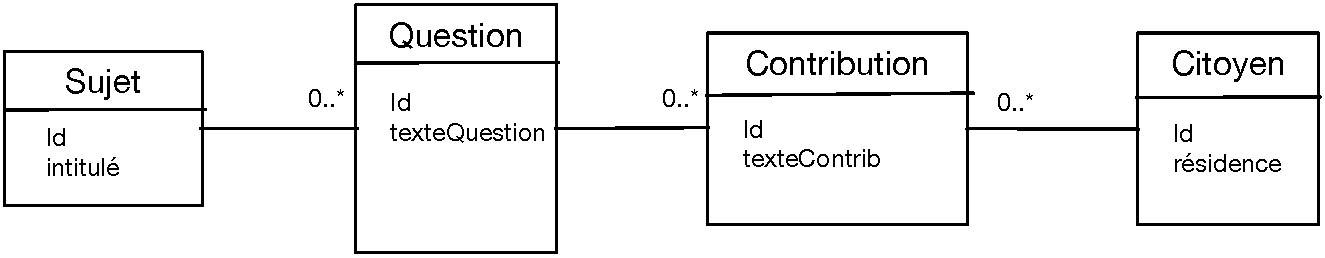
\includegraphics[width=14cm]{schema-granddebat}
  \caption{\label{sgd}  Schéma de la base du Grand Débat}
  \end{center}
\end{figure}

Les contributions sont stockées dans un base relationnelle dont le schéma est donné
par la figure~\ref{sgd} en UML. Elles sont publiées ensuite
sous la forme de documents JSON à des fins d'analyse. 

\begin{enumerate}
  \item Donnez le schéma relationnel correspondant à la figure~\ref{sgd}. 
  \item Donnez un exemple de base relationnelle avec quelques données (très simplifiées) dans chaque table: deux sujets,
      deux questions (une par sujet), trois contributions par deux citoyens. 
      
   \item Donnez une représentation JSON d'un document rassemblant toutes les informations
        (questions, contributions, citoyens) relatives au premier sujet que vous avez choisi.
        
%    \item Donnez une représentation JSON d'un document centré cette fois sur les questions.
    
    \item Indiquez le traitement MapReduce qui permet de passer de la représentation
          précédente à une représentation centrée sur les citoyens.
     
     \item Vous anticipez un très grand nombre de contributions et souhaitez
        donc prévoir un stockage des documents JSON dans un système distribué. Quelle représentation
        vous semble préférable parmi les deux précédentes pour tirer au mieux parti de la distribution\,? 
        
      \item Vous développez un programme \textsc{AnalyseContrib($d$)} qui s'applique à  un
         document $d$ contenant l'ensemble des contributions
          relatives à une question. Quel format ce document devrait-il avoir à
          votre avis pour atteindre une scalabilité maximale\,? 
          Quelle chaîne de traitement permettrait obtenir un tel document
          à partir de l'une des représentations JSON déjà proposées (au choix)\,?
\end{enumerate}

\begin{solution}

\begin{minted}[frame=leftline,
               baselinestretch=.9,
               fontsize=\footnotesize,
               framesep=2mm]{json}
{
  "_id": 978,
  "auteur": "anon102.fr",
  "résidence": "Occitanie",
  "sujet": "Impôts",
  "question": "Payez-vous trop d'impôts?",
  "date": "07/02/2019",
  "titre": "Le président Trump décide d'interdire l'entrée de tout étranger aux USA",
  "contenu": "Suite à un décret paru ....",
  "commentaires": [
     {"internaute": "chocho@monsite.com",
       "note": 5,
       "commentaire": "Les décisions du nouveau président sont inquiétantes ..."
     },
     {"internaute": "alain@dugenou.com",
       "note": 2,
       "commentaire": "Arrêtons de critiquer ce grand homme..."
     }
  ]
}
{
  "_id": 54,
  "source": "nimportequoi.fr",
  "date": "07/02/2017",
  "titre": "La consommation de pétrole aide à lutter contre le réchauffement",
  "contenu": "Contrairement à ce qu'affirment les media officiels ....",
  "commentaires": [
     {"internaute": "alain@dugenou.com",
       "note": 5,
       "commentaire": "Enfin un site qui n'a pas peur de dire la vérité ..."
     }
  ]
}
\end{minted}
\end{solution}


\section*{Deuxième partie : comprendre ElasticSearch (8 pts)}

Voici quelques aspects d'Elastic Search qui devraient vous être familiers, 
et d'autres avancés qui n'ont pas été abordés en cours

\subsection*{Indexation}

La documentation nous dit\,:
\textit{When you index a document, it is stored on a single primary shard determined by a simple formula\,:}

    $$shard = hash(id) \%\ \rm{number\_of\_primary\_shards}$$
    
Voici la configuration de votre \textit{cluster} ElasticSearch pour les questions qui suivent.
Nb\,: réplica = $n$ signifie $n+1$ copies d'un document.

\begin{smallverbatim}
cluster.name: philippe
index.number_of_shards: 3
index.number_of_replicas: 2
\end{smallverbatim} 
Et je crée un index. Chacune des questions ci-dessous vaut 1 point. Une brève explication sera appréciée.

\begin{enumerate}
       \item Comment va réagir Elastic Search à votre avis si le \textit{cluster} est constitué d'un seul n{\oe}ud\,?
       \item Quelle(s) action(s) est/sont nécsessaire(s) si on veut étendre le nombre de \textit{shards}\,?
       \item Quelle(s) action(s) est/sont nécsessaire(s)  si on veut étendre le nombre de réplicas\,?
       \item J'ajoute des n{\oe}uds à mon \textit{cluster}\,: que se passe-t-il\,?
       \item A partir de quand devient-il inutile d'ajouter des n{\oe}uds\,?
\end{enumerate}

Un dernier point à gagner. Un de vos collègues vous affirme qu'il vaut mieux
créer un index avec beaucoup de \textit{shards}, pour anticiper la croissance future. Voici
un argument contre ce choix, issu de la documentation\,:
\textit{term statistics, used to calculate relevance, are per shard. Having a small amount of 
data in many shards leads to poor relevance.} 

Comment lui expliqueriez-vous cet argument dans un français clair et concis\,?

\subsection*{Requêtes}

\begin{enumerate}

  \item On effectue une recherche dans un \textit{cluster} ElasticSearch constitué de 10 fragments (primaires), et on veut récupérer
      le résultat par tranches de 10 documents. Combien faut-il récupérer au minimum de documents de chaque 
      fragment pour constituer un résultat correct pour chaque tranche\,? 

  \item Quelle information le coordinateur de la requête
    devrait-il propager à tous les fragments pour que le classement soit correct (oui cette question est liée
    à un extrait de la doc donné précédemment)\,? 

 \end{enumerate}


\section*{Troisième partie : systèmes distribués (3 pts)}

On considère un système Cassandra avec un facteur de réplication $F= 3$ (donc, 3 copies
d'un même document). Appelons $W$ le nombre d'acquittements reçus pour une écriture, $R$ le
nombre d'acquittements reçus pour une lecture.
\begin{enumerate}
 \item 
 Décrivez brièvement les caractéristiques
des configurations suivantes:
\begin{enumerate}
  \item $R=1, W=3$
  \item $R=1,W=1$
\end{enumerate}
\item
Quelle est la formule sur $R, W$ et $F$ qui assure la cohérence immédiate (par opposition
à la cohérence à terme) du système? Expliquez brièvement.
\end{enumerate}

\section*{Quatrième partie : questions de cours (3 pts)}

\begin{enumerate}
  \item Qu'entend-on par "\textit{bag of words}" pour le modèle des documents textuels en
     recherche d'information? 
     
  \item Expliquez la notion de n{\oe}ud virtuel dans la distribution par \textit{consistent hashing}.
  
  \item Une structure de partitionnement par intervalle indexe des fragments contenant des documents.
     Pourquoi ne pas indexer les documents directement? .

\end{enumerate}

\end{document}
